\documentclass{jsarticle}
\usepackage[dvipdfmx]{graphicx}
\usepackage{listings,jlisting}
\usepackage{amsmath}
\usepackage{float}

\title{情報工学実験2 数理計画法 第二回\\
        項目反応理論:1問からの能力値推定}

\author{学生番号4617043 神保光洋}
\date{\today}
\begin{document}
\maketitle

\section{要旨}
  項目反応理論の紹介とこのモデルを用いた場合の受験者の能力値の推定について学習・演習する
\section{目的}
  統計モデルを用いた分析に欠かせない、パラメタの推定方法について、その基本的な技術を習得することを目的とする。
\section{理論}
\subsection{項目反応理論基礎}
項目反応理論では、ある受験者$j$がある項目$i$に正答する$x_{i, j} = 1$確率を以下の式でモデル化する。

$$
  P(x_{i, j} = 1 | {\theta}_{j} a_i, b_i) = P_i(x_{i, j} = 1 | {\theta}_j) = 
  P_i({\theta}_j) = \frac{1}{1 + \exp{-Da(\theta - b)}}
$$

ここで${\theta}_j$は能力者の能力値パラメタ、$a_i$は項目の識別力パラメタ、$b_i$は項目の困難度パラメタ
である。また、$D=1.7$とする。このモデルには以下の特徴がある。

\begin{enumerate}
  \item ${\theta}_j = b_i$の場合、正答率は$50\%$
  \item また${\theta}= b_i$の場合、正答確率は$50\%$
  \item $a_i = 1, b_i = 0$のとき、この関数は累積標準分布の良い近似となる。
\end{enumerate}


$a$は識別パラメタと呼ばれ、$a$が$0$に近い項目は、
能力値によらず一定の正答率となるような、能力に関係ない項目となる。

項目反応関数は$a$が0に近い値の時は。、能力値に関わらず正答率が高い傾向がある。

また$b$は項目反応関数の正答率が$50\%$ となる$\theta$ の値であり、bが大きな項目では
正答に必要な能力が大きくなる。困難度パラメタと呼ばれるパラメタである。

また、bが大きいほど、小さい能力値での正答率が低い傾向がある。
正答率が$50\%(0.5)$の時の能力値$\theta$の値に着目すると、$b$の値と一致
することがわかる。

\subsection{最尤推定を用いた受験者能力の推定}
項目反応理論を用いた受験者の能力値の推定も1.2節での例と同様に計算する。例えば、今ある問題
に正答した($x_{i, j} = 1$) としよう。この時の受験者の能力値は以下の数式を考えれば良い。

\begin{eqnarray*}
  \hat{(\theta)} = &\arg \max& P(\theta | x_{i, j} = 1) \\
                 & \theta &
\end{eqnarray*}

ただし、$P({\theta}_j | x_{i, j} = 1)$ はIRTのモデルにしたがって、直接は与えられていない
ため、ベイズの定理より、$P_i(x_{i, j} = 1 | {\theta}_j)$を用いて考える。

$$
  P({\theta}_j | x_{i, j} = 1) = \frac{P({\theta}_j)}{P(x_{i,j} = 1)} P_i(x_{i,j} = 1 | {\theta}_j)
$$

ここで、$P(x_{i,j} = 1)$はその問題に正答できる確率であるが、変数${\theta}_j$と独立な変数であるため、
$\arg \max$ を考える上で定数とみなすことができる。したがって、以下の式を考えても結果は変わらない。
 

 \begin{eqnarray*}
   \hat{\theta} = &\arg \max& P(\theta | x_{i, j} = 1) \\
                  &\theta& \\
                = &\arg \max& P(\theta)P_i(x_{i,j} = 1 | {\theta}_j) \\
                  &\theta&
 \end{eqnarray*}

 ここで$P(\theta)$は能力値が一般にどのような分布をしているかを表すので、
 標準正規分布していると仮定できる。

$$
  P(\theta) = \frac{1}{\sqrt{2 \pi}} \exp(- \frac{{\theta}^2}{2})
$$

また、誤答した場合も同様に以下のように考えることができる。

\begin{eqnarray*}
  \hat{(\theta)} &=& \underset{\theta}{\arg \max} P( \theta | x_{i,j} = 1) \\
                 &=& \underset{\theta}{\arg \max} P( \theta ) P_i(x_{i,j} = 1 | {\theta}_j) \\
                 &=& \underset{\theta}{\arg \max} P( \theta ) P(1 - P_i(x_{i,j} = 1 | {\theta}_j))
\end{eqnarray*}

このような関数を考えることで、ある問題に正答、あるいは誤答した場合の学習者の能力値を推定すること
が可能である。また、$P(\theta)$は問題に正答したという事実を受け取る前の確率であり、
事前確率と呼ばれることがある。加えて、$P(\theta | x_{i,j})$
は問題に正答あるいは誤答してという事実を受け取った後の確率なので、事後確率と呼ばれることがある。

また、項目反応理論では、項目情報関数と呼ばれる指標が非常に重要となる。
項目情報量関数とは、項目反応関数について項目への反応から能力値を推定する際のフィシャー情報量
を算出したものであり、2パラメタロジスティックモデルでは以下のような式となる。

$$
  I_i(\theta) = D^2a^2_iP_i(\theta)(1 - P_i(\theta))
$$

フィシャー情報量は一般に$\hat{\theta}$ の標準誤差$se(\hat{\theta})$と以下の関係を持つ

$$
  se(\hat{\theta}) = I_i(\hat{\theta})^{-\frac{1}{2}} = \frac{1}{\sqrt{I_i(\hat{\theta})}}
$$

そのため、この項目情報量を用いることで、推定された$\hat{\theta}$に対してどの程度標準誤差があるか
を見積もることができる

\section{課題}
\subsection{2-1}
課題1-3でといた項目について、表にの特性パラメータを参考に、項目反応関数の
概要を描け。

項目関数は以下のうようになった

\begin{figure}[H]
  \centering
  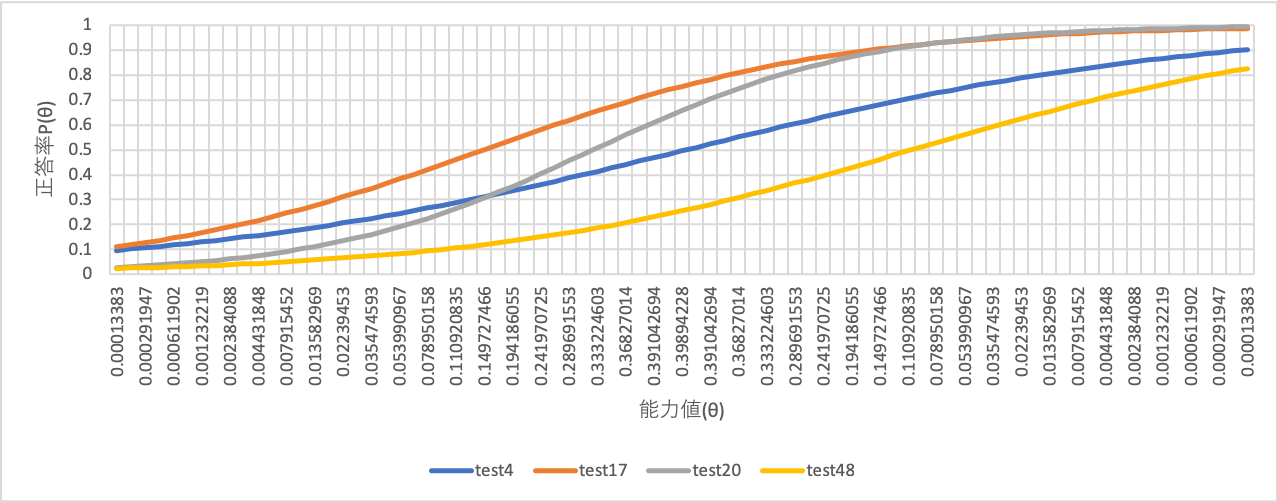
\includegraphics[width=12cm]{./key1.png}
  \caption{項目反応関数}
\end{figure}

\subsection{2-2}
課題2-1で描いたグラフを参考に、それらの項目がどのような項目であったのか
考察せよ。

test48のグラフは能力値が上がっても正答率が上がらないかつ全体的に
正答率が低いことから難しすぎる問題であったと考察される。

\subsection{2-3}
課題1-3でといた項目から1題選びその正誤から描かれる事後分布のグラフを、表2を参考に示せ。

\begin{figure}[H]
  \centering
  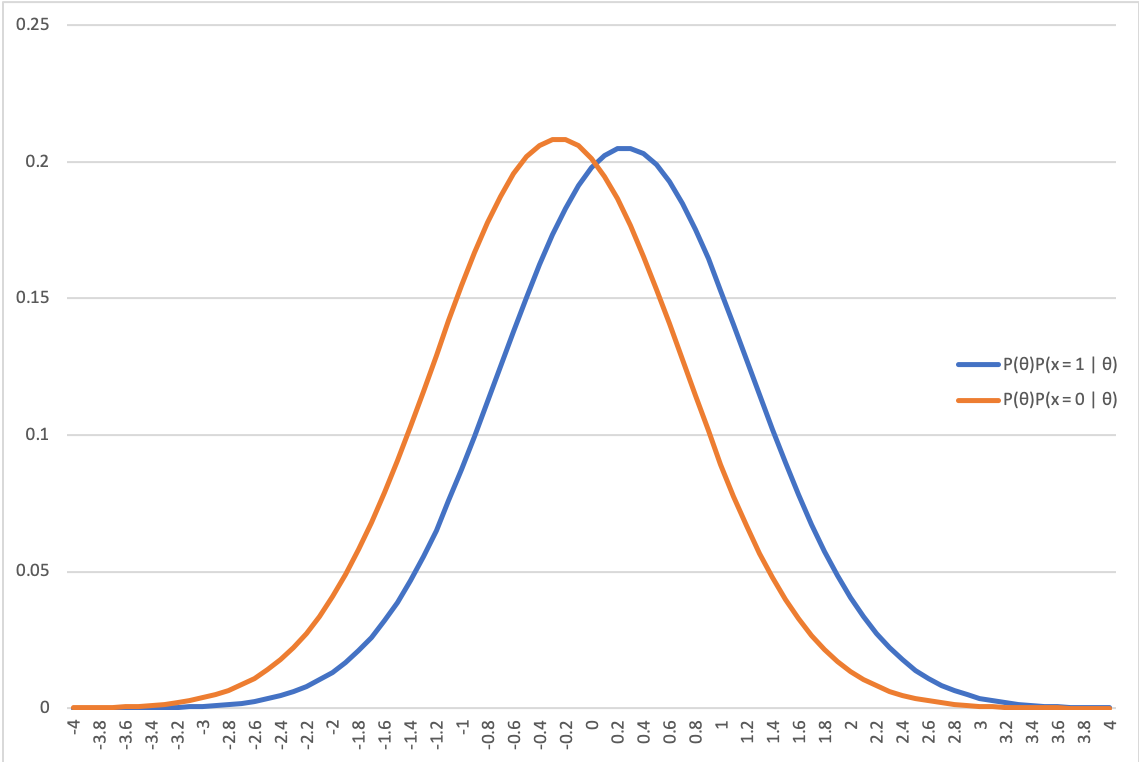
\includegraphics[width=12cm]{./key2.png}
  \caption{事後分布}
\end{figure}

\subsection{2-4}
課題2-3で描いた事後分布から能力値を推定せよ。またその時の標準誤差を求めよ。

    \begin{table}[htb]
      \begin{center}
        \caption{ある大学の学部別、男女別在籍者数の推定結果}
        {\scriptsize
        \begin{tabular}{|c|r|r|} \hline
                                       & 正答時 & 誤答時   \\ \hline
          推定能力値                   & 0.3    & -0.3     \\
          フィシャー情報量 $I(\theta)$ & 0.076  & 0.076    \\
          標準誤差 $se(I)$             & 3.619  & 3.624  \\ \hline
        \end{tabular}
        }
      \end{center}
    \end{table}


\section{参考文献}
\begin{thebibliography}{9}
  \bibitem{key1} 東京大学教養学部統計学教室 統計学入門 (基礎統計学Ⅰ)・東大出版会
\end{thebibliography}

\section{付録}

\end{document}
